\chapter{MDPs}

What is a decision problem?
Why do we care?

\hypertarget{sequential-decision-problems}{%
\section{Sequential decision
problems}\label{sequential-decision-problems}}

% MDPs are a subset of sequential decision problem. Define MDPs. Give
% example.

A MDP is defined as a tuple, \(\{\mathcal S, \mathcal A, P(s_{t+1} \mid s_t, a_t),R(s_t, a_t, s_{t+1}), \gamma\}\)\footnotemark[1]. Where \(s \in \mathcal S\) is the set of possible states (\textit{for example arrangements of chess pieces}), \(a \in \mathcal A\) is the set of actions (\textit{the different possible moves, left, right, diagonal, weird L-shaped thing, ...}),  \(P(s_{t+1} \mid s_t, a_t)\) is the transition function which describes how the environment acts in response to the past (\(s_t\)) and to your actions (\(a_t\)) (\textit{in this case, your opponent's moves, taking one of your pieces, and the results of your actions}), and finally, \(r(s_t, a_t, s_{t+1})\) is the reward function, \textit{whether you won (+1) or lost (-1) the game }.
The objective when solving a MDP is to find a policy, $\pi(a_t | s_t)$, that maximises the discounted cumulative reward, \(R =\sum_{t=0}^T \gamma^t r(s_t, a_t, s_{t+1}) \).

\footnotetext[1]{Why is the discount factor a part of the definition of the MDP?
By defining the discount it ensures the MDP has a unique solution.}

If we wanted we could pick our actions before we make observations,
reducing the search space to only \(|A| \times T\). But this is a bad idea\ldots{} example.

The general feeling of an MDP. - Actions need to be adapted to new
observations and contexts. - While instantaneous results are good, we
care about the longer term aggregates.

\hypertarget{the-markov-property}{%
\subsection{The Markov property}\label{the-markov-property}}

\begin{displayquote}
  What does the M in MDP really mean?
\end{displayquote}

When we say a decision problem is Markovian, we mean that the transition
function generates a Markov chain. The next transition step depends only
on the current state and action. It is invariant to any and all histories that do not
change the current state.

This is not to say that past actions do not effect the future. Rather,
it is a special type of dependence on the past. Where the dependence is
totally described by changes to the \textbf{observable} state.

% Can easily make a sequence Markovian by adding information. E.g.
% time

When actions you have taken in the past can bite you in the butt \ldots{}
Maze with pendulums / doors. When moving through the maze, you must
swing the pendulums. In the future you must avoid being hit. (maybe make
a picture of this?) also, is there a more general way to think about it?

\hypertarget{optimality}{%
\section{Optimality}\label{optimality}}

\begin{displayquote}
  What does it mean to solve an MDP?
\end{displayquote}

And importantly, existing theory tells us that there is a unique optima to the bellman iterations.
And that this optimal policy(ies) is(are) necessarily deterministic.

(why does this make sense?)

\hypertarget{solutions}{%
\subsection{Solution complexity}\label{solutions}}

\begin{displayquote}
  How hard is it to solve an MDP?
\end{displayquote}

% Insert lower bound and some intution

\begin{align*}
Q^{\pi}(s_0, a_0) = r(s_0, a_0) &+ \gamma \mathop{\text{max}}_{a_1} \mathop{\mathbb E}_{s_1\sim p(\cdot | s_0, a_0)} \Bigg[ \\
r(s_1, a_1)  &+ \gamma \mathop{\text{max}}_{a_2} \mathop{\mathbb E}_{s_2\sim p(\cdot | s_1, a_1)} \bigg[\\
r(s_2, a_2)  &+ \gamma \mathop{\text{max}}_{a_3} \mathop{\mathbb E}_{s_3\sim p(\cdot | s_2, a_2)} \Big[
\dots \Big] \bigg] \Bigg]
\end{align*}

\hypertarget{how-do-mdps-relate-to-rl}{%
\section{How do MDPs relate to RL?}\label{how-do-mdps-relate-to-rl}}

Reinforcement learning refers to the set of solutions to a type of problem.
This general, reinforcement learning, problem, has two main properties;
\textit{"trial-and-error search and delayed rewards"} \cite{Sutton2018}.
Unlike supervised learning, which gives the learner feedback (\textit{Student: "I think that digit
is a 5". Teacher: "No, it's a 6"}), in RL the learner only receives evaluations (\textit{Student: "I think
that digit is a 5". Teacher: "No."}). This means the student needs to explore the possible answers via some trial-and-error search.
(\textit{Student: "Is it a 4?". Teacher: "No." Student: "How about a 0?". Teacher: "No." ... Student: "A 6?". Teacher: "Yes."})

Ontop of terse teachers, many actions may be taken
before any evaluation is received, thus requiring credit to be assigned to actions,
often leaving the learner wondering: "what did I do to deserve this?" (see
\href{https://www.youtube.com/watch?v=Qv4H81gEGDQ}{pigeon superstition} for an amusing
example of credit assignment gone wrong \cite{Box1997}).

% Your teaher might only give you evaluations for sequences of actions, rather than individual actions.
% Thus you are left with trying to infer how these sequence evaluations tells you about which actions you should take.

The above definition of reinforcement learning is very general, and there are many
different dimensions to the various RL settings, for example;

\begin{itemize}
\tightlist
\item
  Observable versus non-observable
\item
  Deterministic versus stochastic
\item
  Synchronous versus asynchronous
\item
  Terminating versus infinite
\item
  Knowledge of the model
\item
  Discrete versus continuous
\end{itemize}


MDPs are also within the fields of Operational Research, Optimal Control, Mathematical
Optimisation, Stochastic Programming.



\hypertarget{a-tabular-representation-of-mdps}{%
\subsection{A tabular representation of MDPs}\label{a-tabular-representation-of-mdps}}

\begin{displayquote}
  What is the minimally complex setting we can consider that still poses an
  interesting challenge to the ML / RL communities?
\end{displayquote}

Let start with a tabular MDP. We can describe the MDP with tables, a table for the transition probabilities,
a table for the rewards. discrete states and
actions - \(r\) and \(P\) are simply look up functions, indexed by the
current state-action.

Consider a tabular MDP with deterministic actions, $P(s_{t+1}|s_t, a_t) \in \{ 0, 1\}$.
It can be efficiently solved by non-statistical
methods: dynamic programming (ref) and related planning techniques (ref).

But a tabular MDP with stochastic actions, $P(s_{t+1}|s_t, a_t) \in [0, 1]$,



A result of this formulation is that we consisely write and solve the Bellman equation.

\begin{align}
V &= r_{\pi} + \gamma P_{\pi} V \tag{the bellman eqn}\\
V - \gamma P_{\pi} V &= r_{\pi}\\
(I-\gamma P_{\pi})V &= r_{\pi}\\
V &= (I-\gamma P_{\pi})^{-1}r_{\pi}
\end{align}

Where $r_{\pi}[s, a] =  \pi[s, a] r[s, a], P_{\pi}[s', s] = \sum_a P[s', s, a]\pi[s, a]$.

\section{The value function polytope}

The value function polytope \cite{Dadashi2018} is the
Why is it a polytope?

Imagine a two state MDP. Following some initial, ill-informed policy,
the value that you might get starting from either state state is $v_1, v_2$.



\begin{figure}
\centering
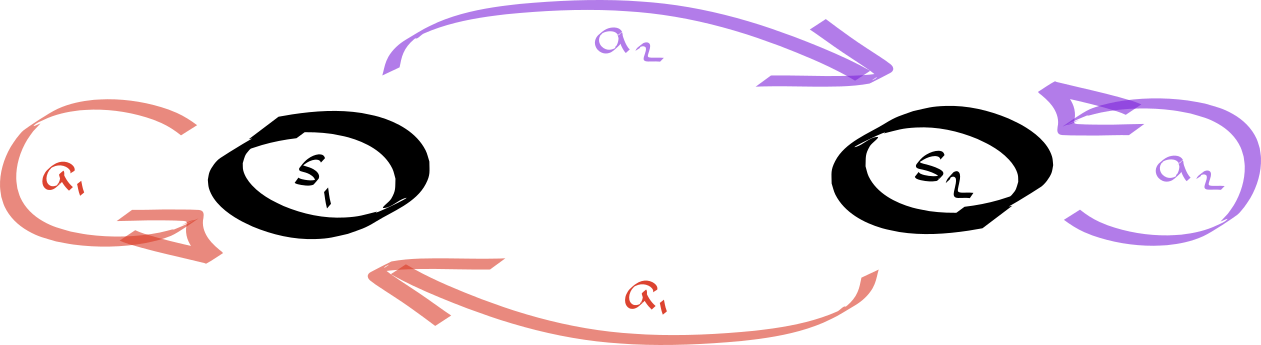
\includegraphics[width=1\textwidth,height=0.25\textheight]{../../pictures/drawings/2-state-automata.png}
\caption{Consider the simplest possible MDP, with two states and two actions. (Any simpler setting is entierly uninteresting. A single state means actions do nothing.
And a single action means all policies are the same...).}
\end{figure}


% \begin{figure}
% \centering
% 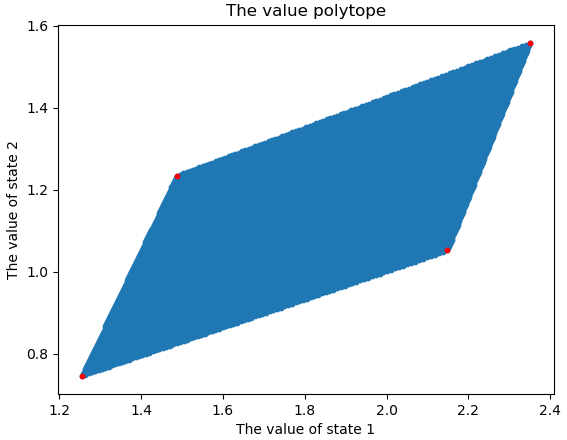
\includegraphics[width=1\textwidth,height=0.25\textheight]{../../pictures/drawings/value-polytope.png}
% \caption{The value polytope for a two state, two action MDP.}
% \end{figure}

\subsection{What are the properties of the polytope?}

\begin{displayquote}
  How is the structure of the RL problem reflected in geometry?
\end{displayquote}

How is the shape of the polytope determined by the Bellman equation?
If we look at the polytope, we see that;
\begin{itemize}
\tightlist
\item
  All the edges have positive gradients
\item
  All the edges are linear
\item
  Non-convex
\end{itemize}


% An increase in the value of state one, can, at worst, do nothing for state two, aka a
% flat line, either horizontal or vertical. But if the value of the other state
% increases and there is a non zero chance of transitioning to that state, from your current state,
% then that will increase the value of your current state.
% This explains why the edges of the polytope by be aligned with the positive orthant, they slant upward.

\begin{align}
\hat V(s_1) = V(s_1)P(s_1|s_1, a)\pi(a|s_1) + V(s_2)P(s_2|s_1, a)\pi(a|s_1)
\end{align}

\begin{itemize}
\tightlist
\item
If $V(s_1)$ increases then $\hat V(s_1)$ must increase...
\item
If $V(s_2)$ increases then $\hat V(s_1)$  either increases or stays the same. As $P(s_2|s_1, a)\pi(a|s_1) \ge 0$
\end{itemize}

\subsection{Policies in high dimensions}



\begin{figure}
\centering
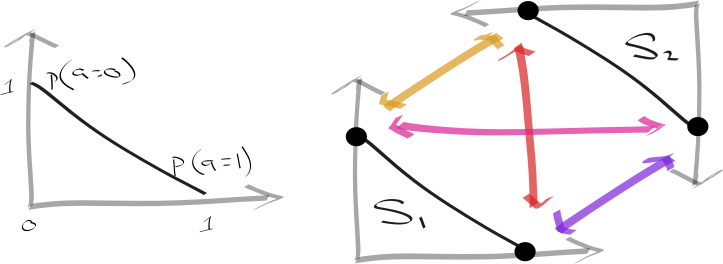
\includegraphics[width=1\textwidth,height=0.25\textheight]{../../pictures/drawings/2-state-2-action-simplices.png}
\caption{Imagine what the geometry of the space of policies in the two state, two action MDP. A policy tells us what actions should be taken when in a given state. Therefore, there will be \(|A| \times |S|\) entries in the policy. However, because the policy returns a distribution over actions, the true dimensionality of the policy is \((|A| -1) \times |S|\). Which in the two state, two action case equals 2D.}
\end{figure}

\begin{figure}
\centering
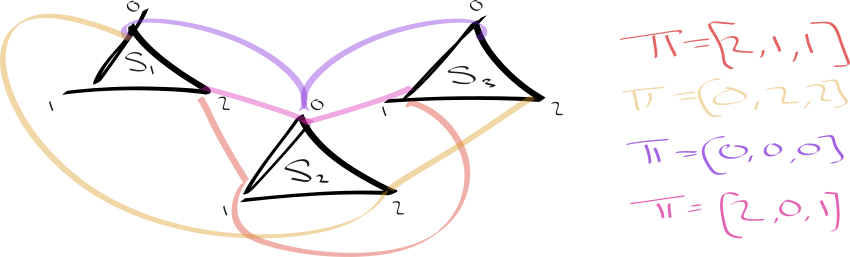
\includegraphics[width=1\textwidth,height=0.25\textheight]{../../pictures/drawings/3-state-3-action-simplices.png}
\caption{Let's \textit{try} to gain some intuition about the space of policies in higher dimensions.
For each state, we have a distribution (on a simplex), over the possible actions.}
\end{figure}

\section{Search spaces}

Overview.
Mention cts relaxations!?
Relation to the deep learning puzzle of over parameterisation.

\subsection{Dynamics and complexity}

\textbf{TODO} Complexity. How many iterations!!! Look up from literature
and do some empirical tests.

(we want to know how much it costs to find the optima)

For each initial policy, we can solve / optimise it to to find the
optimal policy (using policy iteration). Here we count how many
iterations were required to find the optima (from different starting
points / policies).

Policy iteration can be summarised easily as an iteration between
evaluation and updates, see below.

\begin{verbatim}
pi = init
while not converged:
  value = evaluate(pi)
  pi = greedy_update(value)
\end{verbatim}

\begin{figure}
\centering
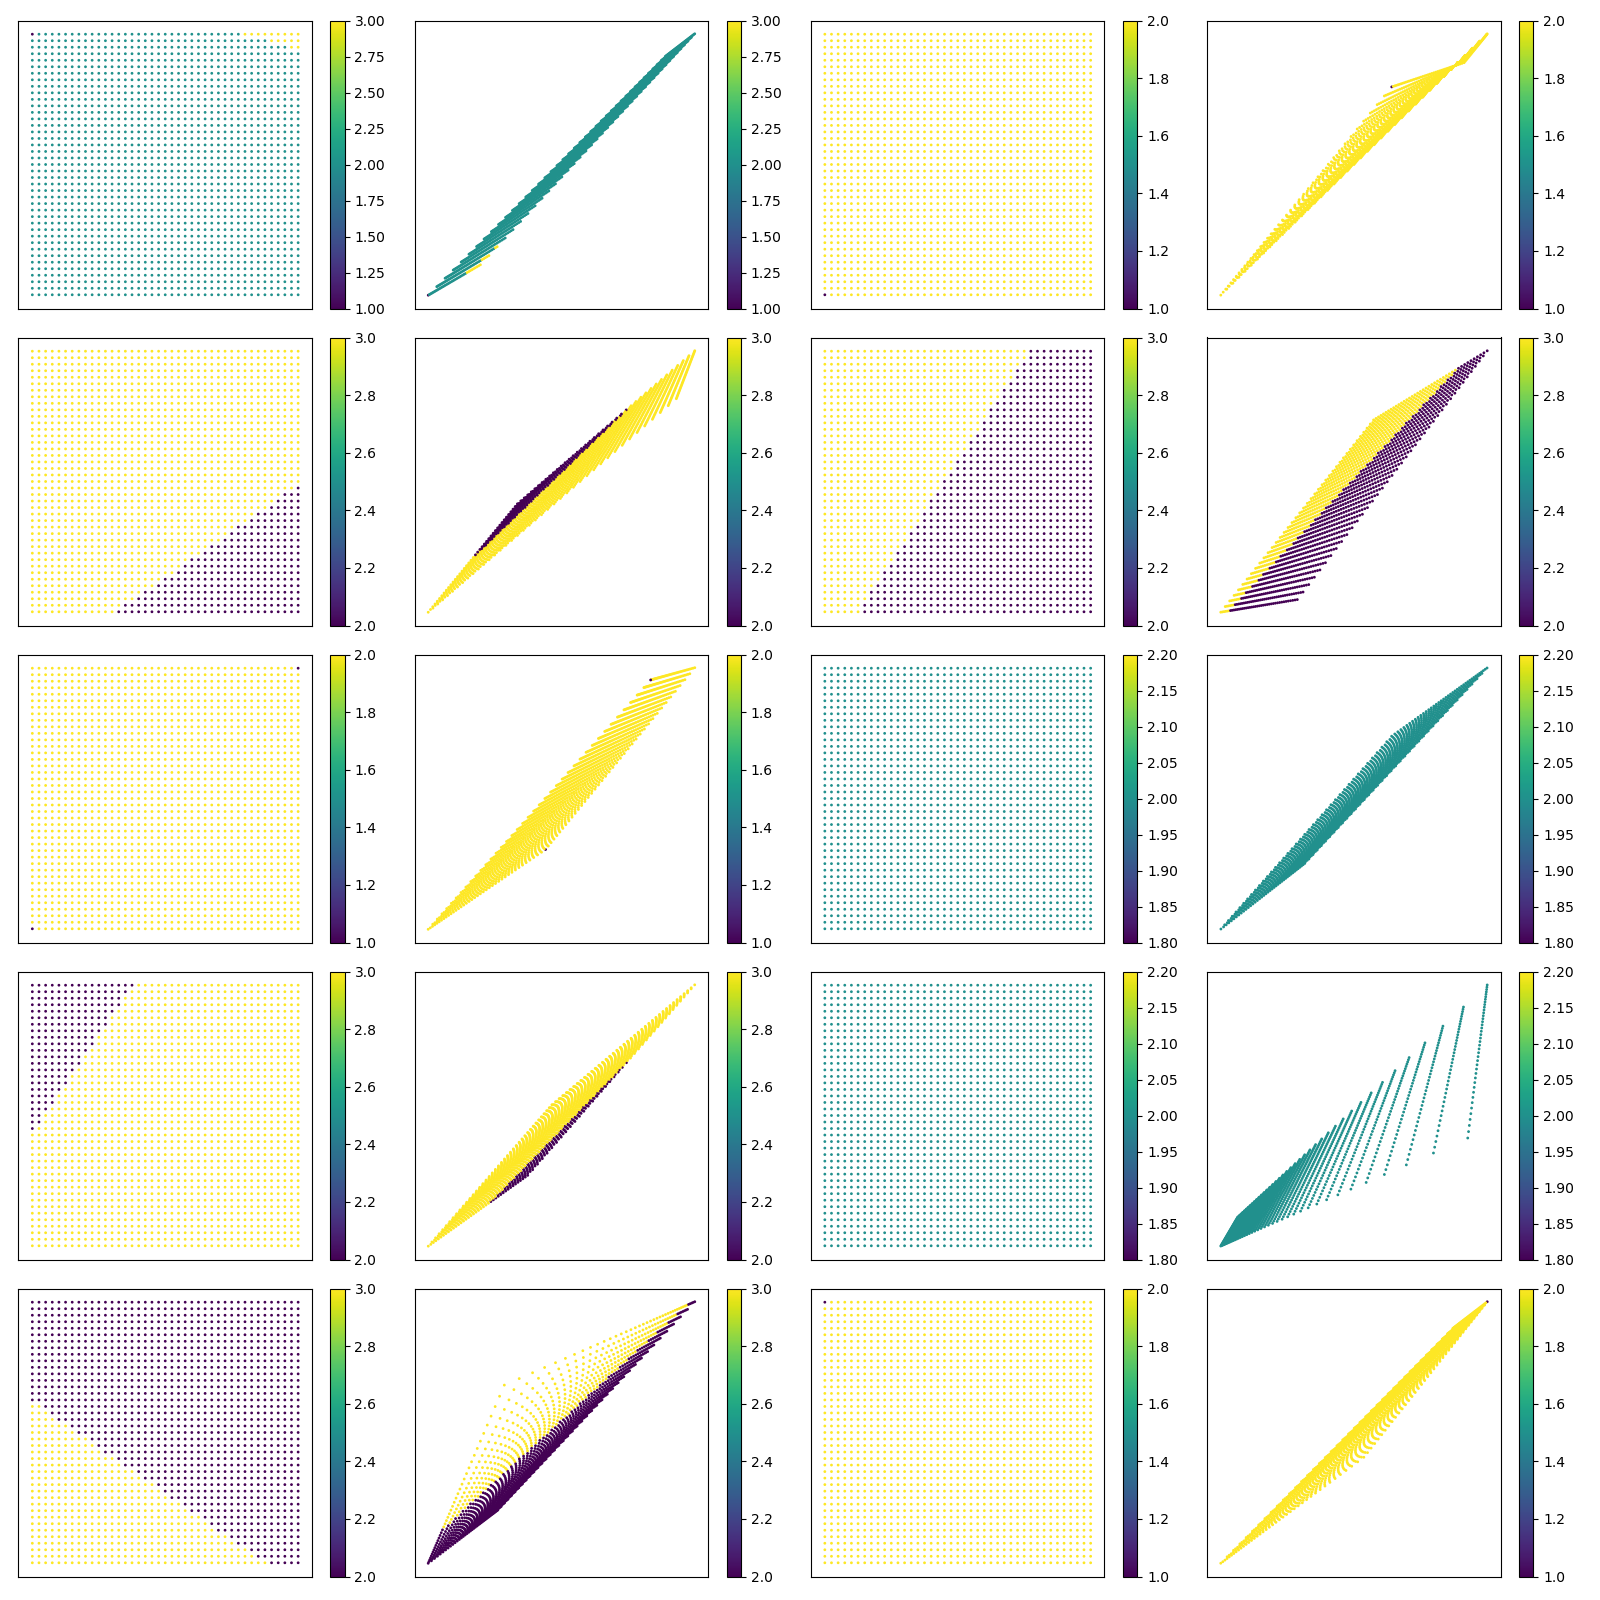
\includegraphics[width=0.5\textwidth,height=0.5\textheight]{../../pictures/figures/gpi-partitions.png}
\caption{`2-state 2-action MDPs. We have visualised the number of steps
required for convergence to the optimal policy. The number of steps are
show by color.'}
\end{figure}

\begin{itemize}
\tightlist
\item
  What are the best ways to travel through policy space? (lines of
  shortest distance?!)
\item
  How does this scale with \texttt{n\_actions} or \texttt{n\_states}??
\item
  Is there a way to use an interior search to give info about the
  exterior? (dual methods?!)
\item
  What if your evaluations are only \(\epsilon\)-accurate? How does that
  effect things?!?
\end{itemize}

\subsection{Efficient search}

We want to efficiently find the optimal policy for a given MDP. But where and how should we
search for this policy? We could search within;

\begin{itemize}
\tightlist
\item
the set of potentially optimal policies, the \(|A|^{|S|}\) discrete policies,
\item
the set of possible value functions, \(\mathbb R^{|S|}\),
\end{itemize}
or maybe some other space. But which space is best?

% Which space allows us to find the optimal policy in the 'cheapest' manner?
Naively, we know that smaller search spaces are better. We would rather
search for our keys in a single room, rather than many. But added
structure (for example, continuity) can be exploited to yield faster
search, even when there are infinitely more states to search.
% want example!?

% Aside. Deep learning - search space. Overparameterisation. \cite{Arora2018}

% need a better seguae into GD?!
Let's focus on searching with gradient descent.

\begin{align}
w_{t+1} = w_t - \eta \nabla f(w_t) \\
\end{align}

The dynamics of the search are dependent on the topology of a problems loss surface.
The loss surface is determined by the combination of the search space and the loss function.

\begin{align}
&\mathop{\text{max}}_V \mathop{\mathbb E}_{s\sim D} V(s) \\
&\mathop{\text{max}}_{\pi} \mathop{\mathbb E}_{s\sim D}V^{\pi}(s) \\
&\mathop{\text{max}}_{\theta} \mathop{\mathbb E}_{s\sim D} V_{\theta}(s) \\
&\mathop{\text{max}}_{\theta} \mathop{\mathbb E}_{s\sim D} V^{\pi_{_{\theta}}}(s) \\
&\mathop{\text{max}}_{\phi} \mathop{\mathbb E}_{s\sim D} V^{\pi_{_{\theta_{\phi}}}}(s) \\
&\mathop{\text{max}}_{\varphi} \mathop{\mathbb E}_{s\sim D} V^{\pi_{_{\theta_{\phi_{\varphi}}}}}(s)
\end{align}

We can pick any space we we like to search with in. But, why would we want to pick one space over another?

\begin{itemize}
\tightlist
\item
  In which spaces can we (efficiently) calculate gradients?
\item
  In which spaces can we do convex optimisation?
\item
  In which spaces does momentum work (well)?
\end{itemize}


\subsection{Value search}

Value iteration versus deep value.

In RL it is possible to transform the hard combinatorial problem of
searching through the \(|A|^{|S|}\) possible discrete policies, into an
easier (how do we know it is easier?!? PROOF) problem, a search through
all possible policies \(?!?\).

Intution about why it converges!?

\cite{Bellman1957}

\subsection{Policy search}

\begin{align}
\pi^{* } = \mathop{\text{argmax}}_{\pi} V(\pi)
\end{align}

Policy iteration versus PG.

When transforming between two spaces, how does the optimisation space
change? Does my abstraction make optimisation easier?

add ref

\subsection{Model iteration}

Search through possible models, \(\tau, r\), calculate the optimal
policy \(\pi^{* }_{\tau, r}\) and then update \(\tau, r\) based on
\(\parallel V_{\tau, r}(\pi^{* }) - V(\pi^{* }) \parallel\).

Search through models while trying to find one that yields similar returns to the oracle when playing the same policy.
A supervised problem...

\begin{align}
\theta^{* } = \mathop{\text{argmin}}_{\theta} \int_{\Pi} \parallel V^{\pi}_{P, r} -V^{\pi}_{\theta} \parallel_2
\end{align}

Note this solver is different to the others. In the previous optimisations we assumed that we knew the model.

% Related to;
% - Thompson sampling?!?
% - invaraint risk minimisation
% - compressed sensing. each policy is one of our sampling bases!? rather than using the deterministic policies (the pixels), we can use mixtures!?

Once we have the model, we can solve for the optimal policy.

Relation to model based RL. This algol only focuses on relevant features of the state space.
Where model base learners that attempt to learn by predicting transitions can be made to scale arbitrarily worse.
Consider a problem where the reward is only determined by the first feature of the state. We can add $n$ extra, useless, features.
The model based learner will spend resources on attempting to build a good predictor of those $n$ features.

Sample efficient. You only need to collect data for the $m$ policies we are matching under.
Once that has been done, the optimisation problem is easily solved!?

Model iteration. Model invariant transforms. Pick a policy. Falsify it,
and this falsify all models that yield the same optimal policy.

\begin{figure}
\centering
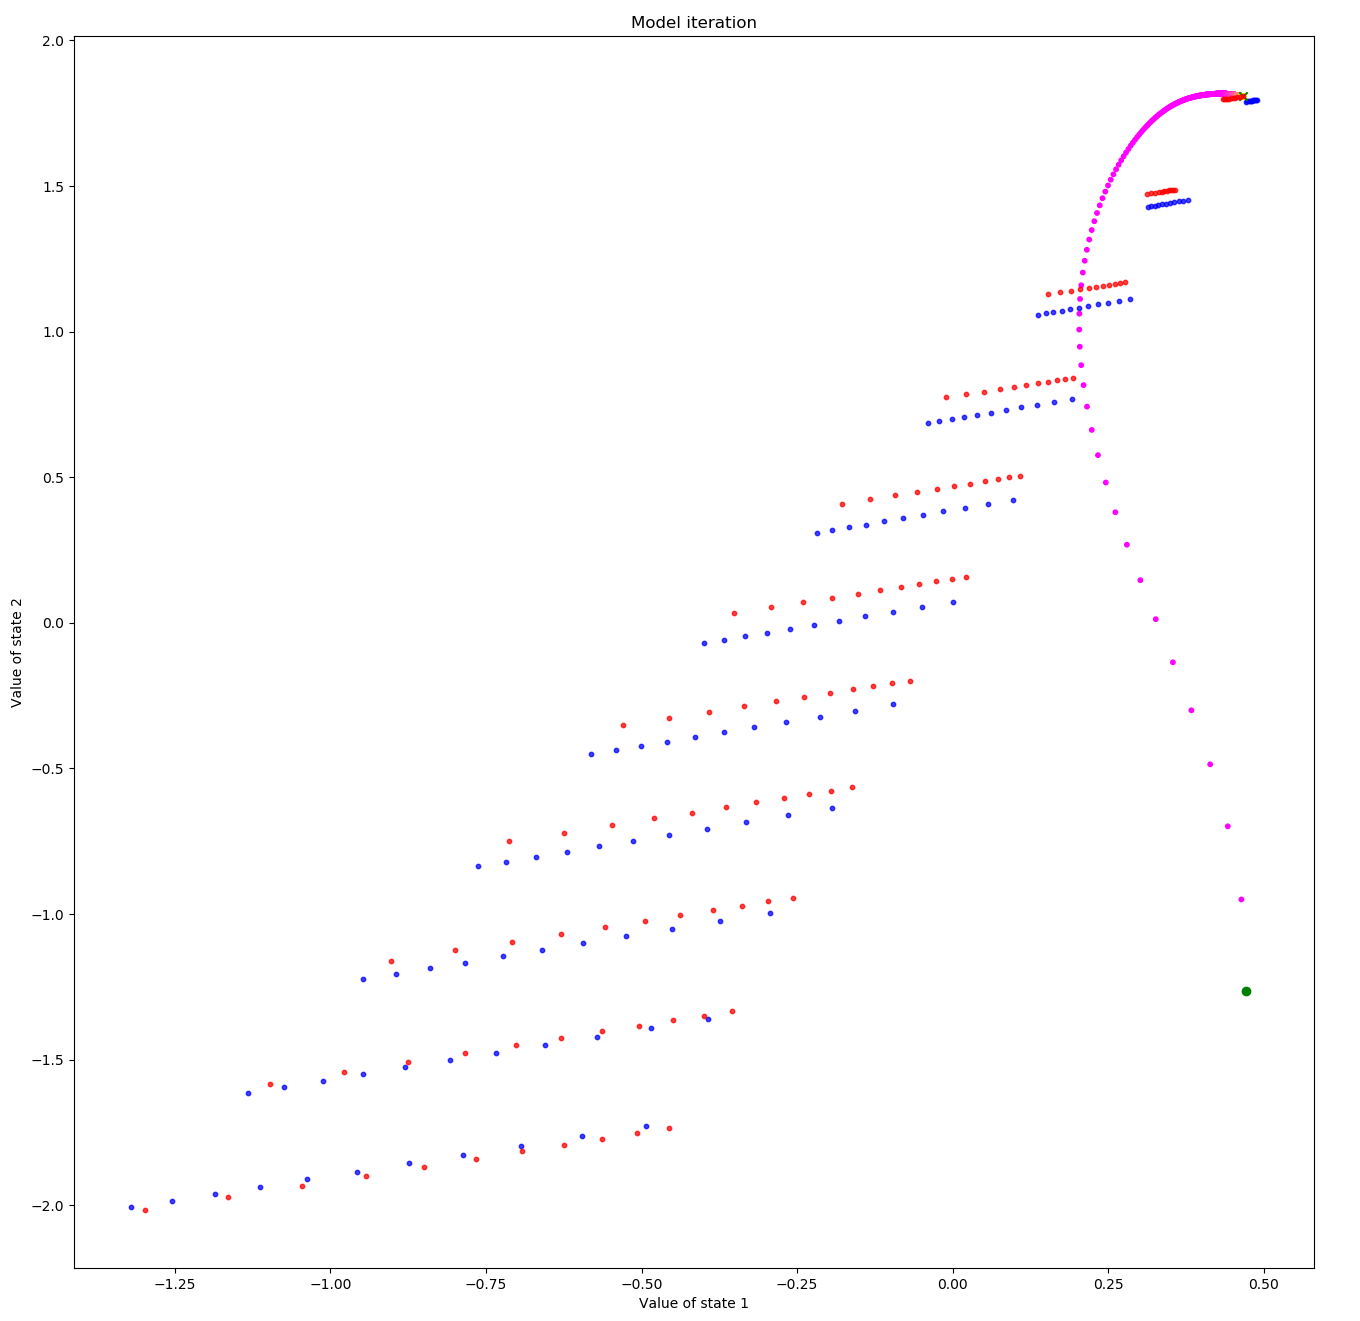
\includegraphics[width=0.5\textwidth,height=0.5\textheight]{../../pictures/figures/model_iteration.png}
\caption{Blue shows the value of policies when evaluated under the true model, $P, r$,
and Red shows the value of policies when evaluated under the learned model at convergence.}
\end{figure}


Related to AWR? https://arxiv.org/pdf/1910.00177.pdf

\subsection{Topology and dynamics}

Ok, so if we parameterise our search space. We have now changed the
topology of our search space.

\textbf{Q:} How can we rationally pick the topology of our search space
to accelerate learning?

\begin{itemize}
\item
  A well connected space? For all possible policies, there exists
  \(\theta_1, \theta_2 \text{ s.t. } \parallel \theta_1- \theta_2\parallel_2\)
  is small. (but that doesnt necessarily help\ldots{} depends on the
  landscapce imposed by \(\nabla_{\theta} V\))
\item
  ???
\end{itemize}

See these gradient flows for example;

Pics?!?

Here are some examples \ldots{}???

\begin{figure}
\centering
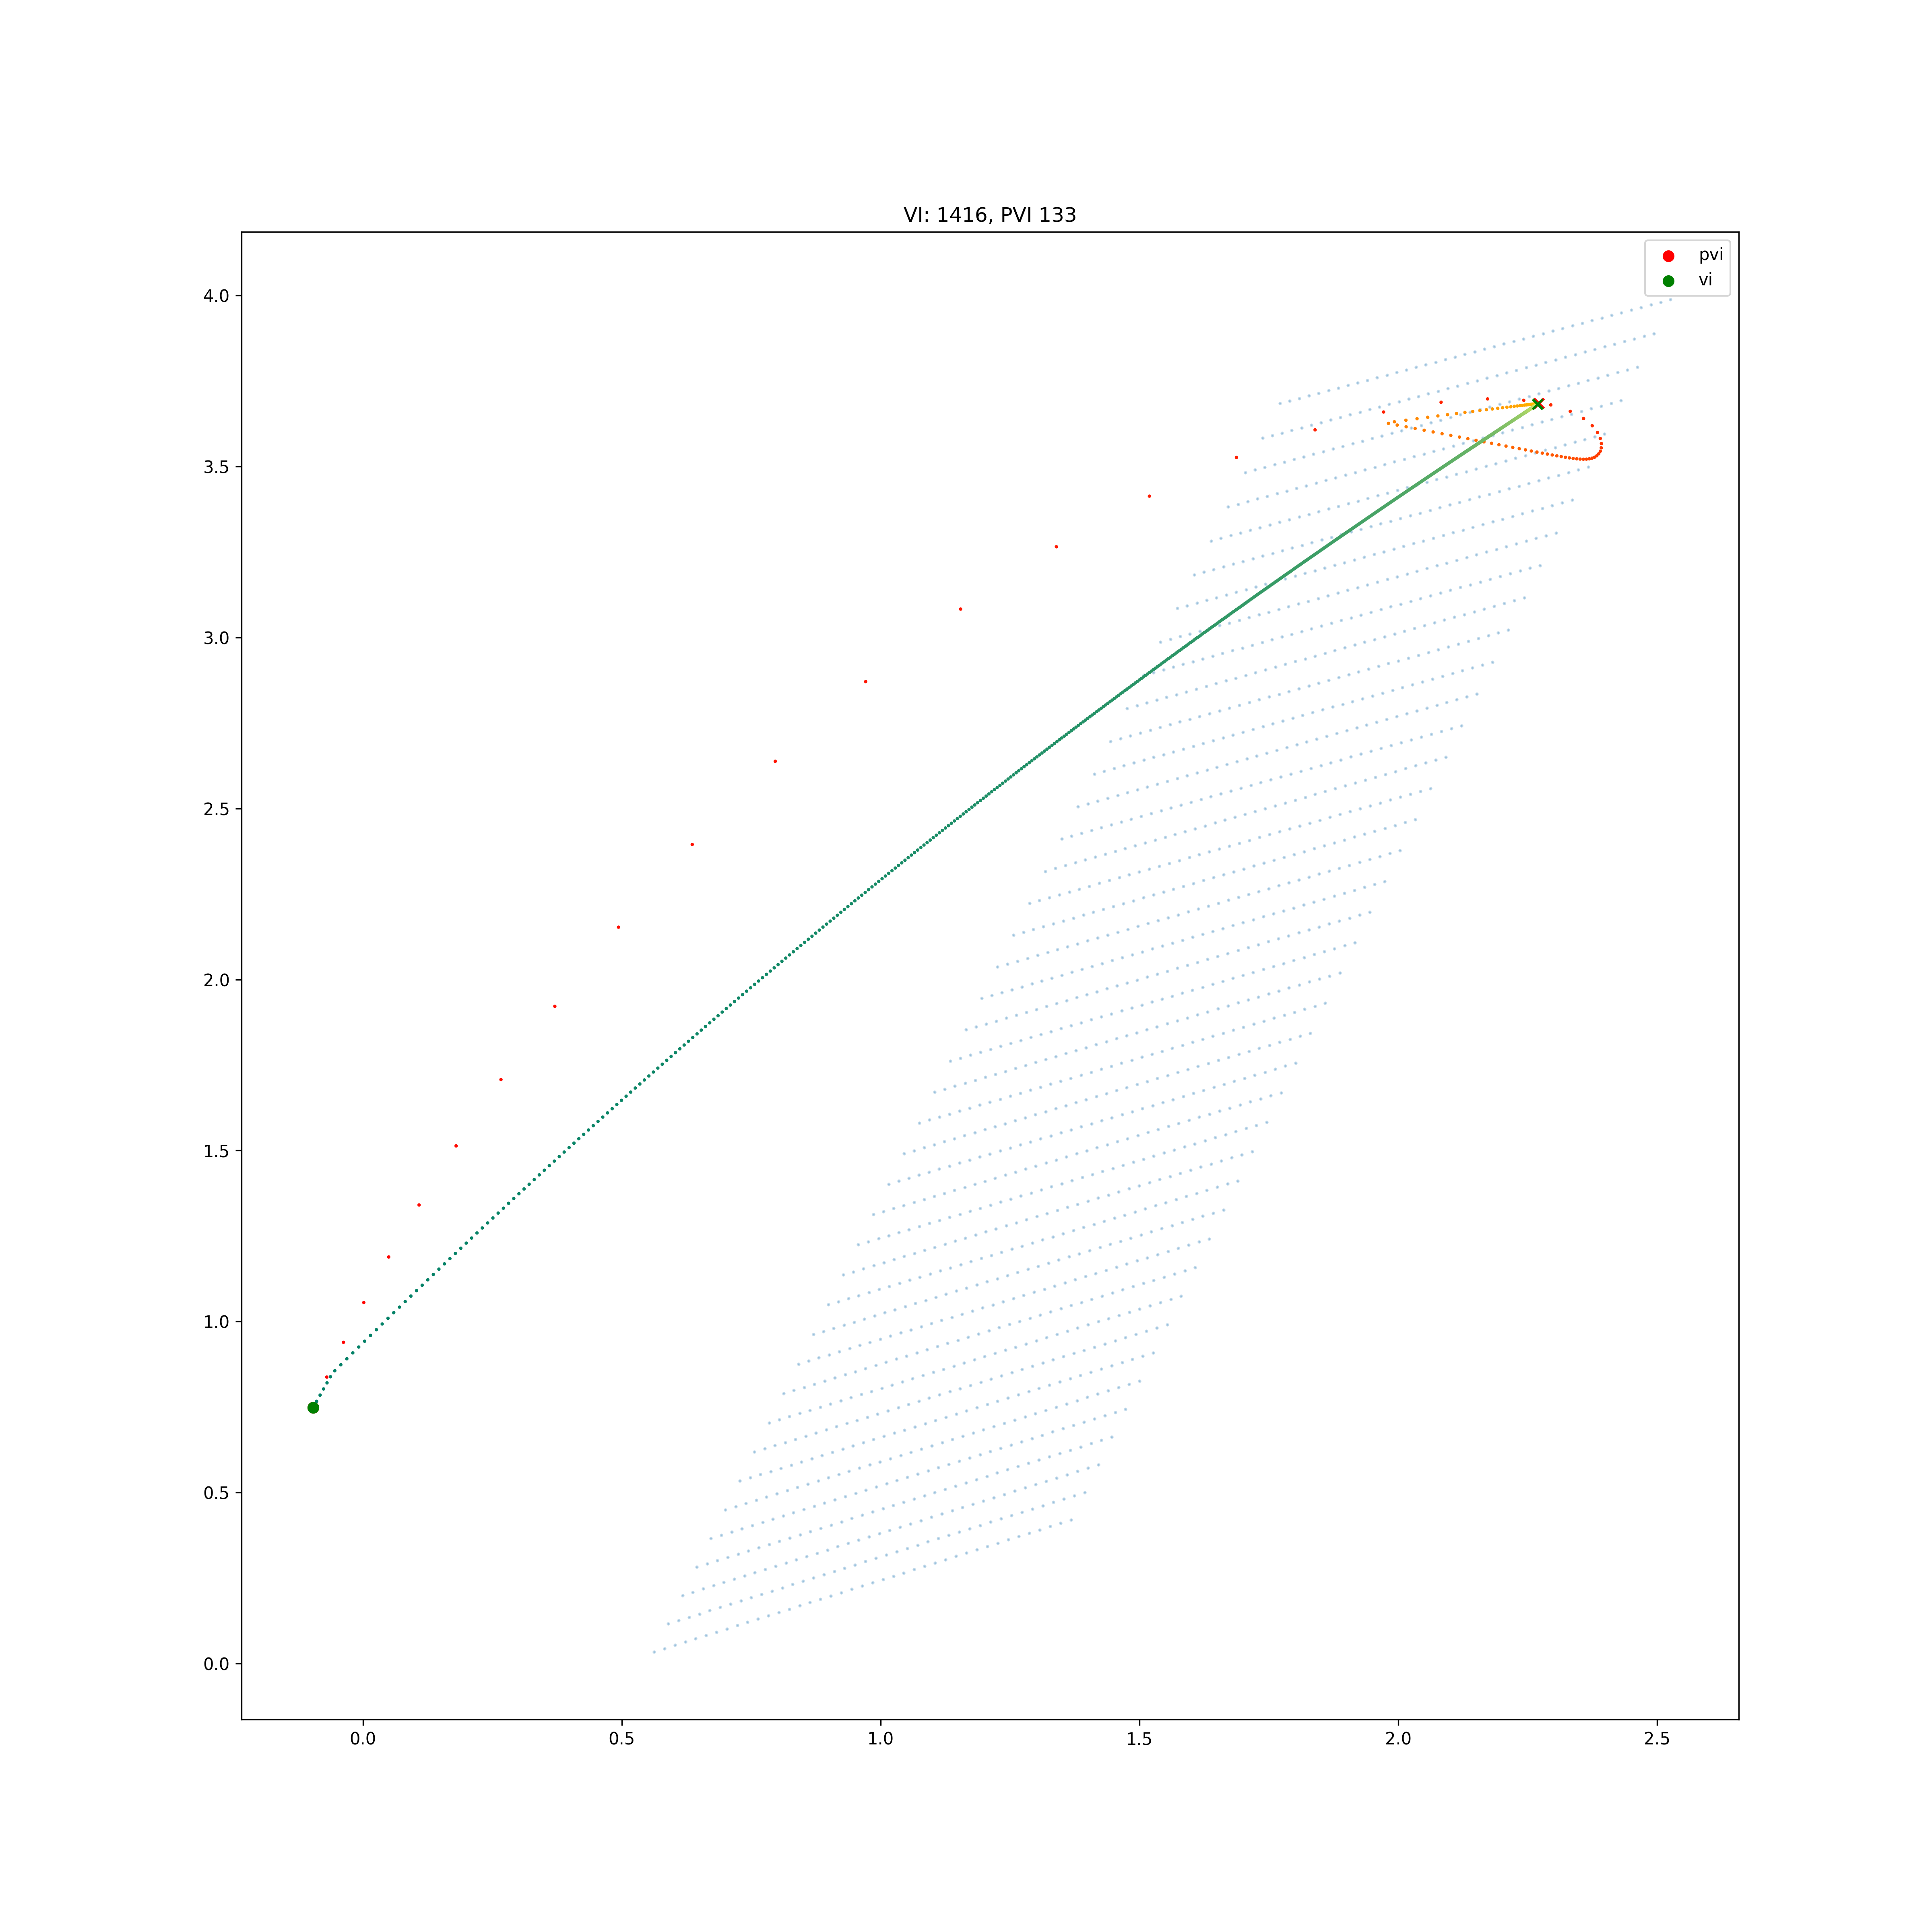
\includegraphics[width=0.5\textwidth,height=0.5\textheight]{../../pictures/figures/vi-vs-pvi.png}
\caption{The optimisation dynamics of value iteration versus parameterised value iteration.}
\end{figure}

\begin{figure}
\centering
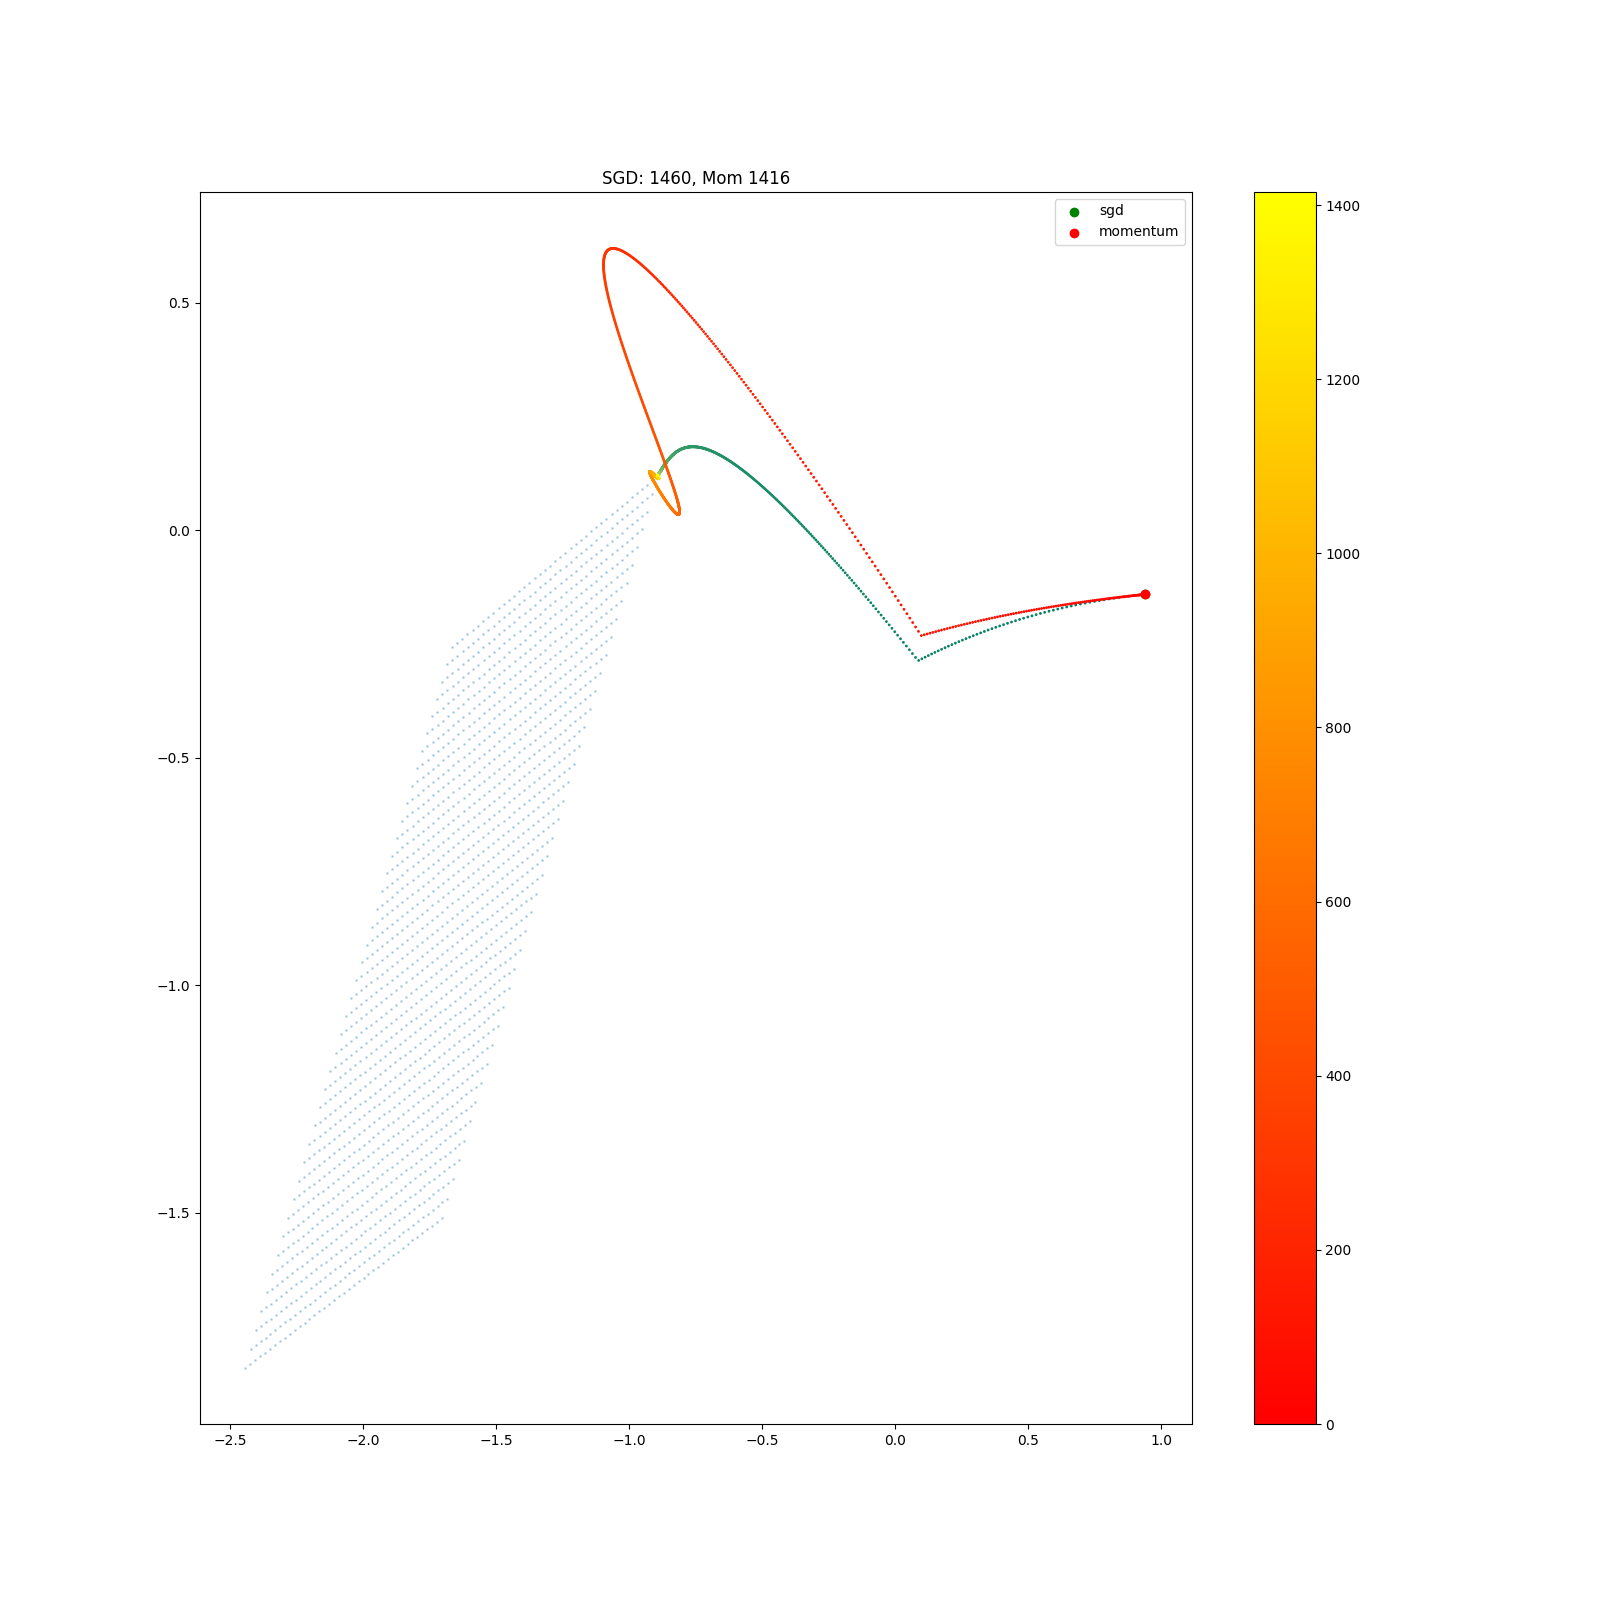
\includegraphics[width=0.5\textwidth,height=0.5\textheight]{../../pictures/figures/vi_sgd-vs-vi_mom.png}
\caption{The optimisation dynamics of value iteration versus value iteration with momentum.}
\end{figure}

If we overparameterise the search space, then we can move between solutions in new ways. We can `tunnel' from A to B, without crossing C.
%  insert pic / prove

Every point (in output space) is closer, when measured in the distance in parameter space needed to be traveled.
% insert pic / prove

\subsection{Acceleration and parameterisation}

I think something weird happens with momentum in overparameterised spaces. The intuition is

\cite{Arora2018} shows that overparameterisation yields acceleration. Consider
the dynamics of the parameter $w$, which we have overparameterised as $w_1 \cdot w_2$.

\begin{align}
w^{t+1} &= w_1^{t+1} \cdot w_2^{t+1} \\
&= (w_1^t - \eta \nabla_{w_1} L)\cdot(w_2^t - \eta \nabla_{w_2} L) \\
&= (w_1^t \cdot w_2^t - \eta w_2^t \nabla_{w_1} L - \eta w_1^t \nabla_{w_2} L - \mathcal O(\eta^2) \\
&= w^t - ...
\end{align}

We have implicit momentum from the parameterisation, and explicit momentum in the accelerated descent.


\begin{align}
m_{t+1} &= \gamma m_t + g_t \\
w_{t+1} &= w_t - \eta \cdot (1-\gamma) \cdot m_t
\end{align}

It is necessary to consider the trajectory to study momentum. It depends
on what has happened in the past. Can we construct a space of possible
trajectories? What properties do trajectories have? They are connected
by the update fn.

Set $g_t = \rho(t) \nabla_w + \sum_{\tau=0} \mu g_{\tau}$.

\begin{align}
m_{t+1} &= \gamma m_t + \rho(t) g_t + \sum_{\tau=0} \mu_{\tau, t} g_{\tau} \\
w_{t+1} &= w_t - \eta \cdot (1-\gamma) \cdot m_t \\
&= w_t - \eta \cdot (1-\gamma) \cdot \sum_{k=0}^t \gamma^{t-k}\big[ \rho_t g_k + \sum_{\tau=0} \mu_{\tau, k} g_{\tau} \big]
\end{align}

\subsection{Continuous flow and its discretisation}

A linear step of size, \(\alpha\), in parameter space, ie by gradient
descent, is not necessrily a linear step in parameter space.

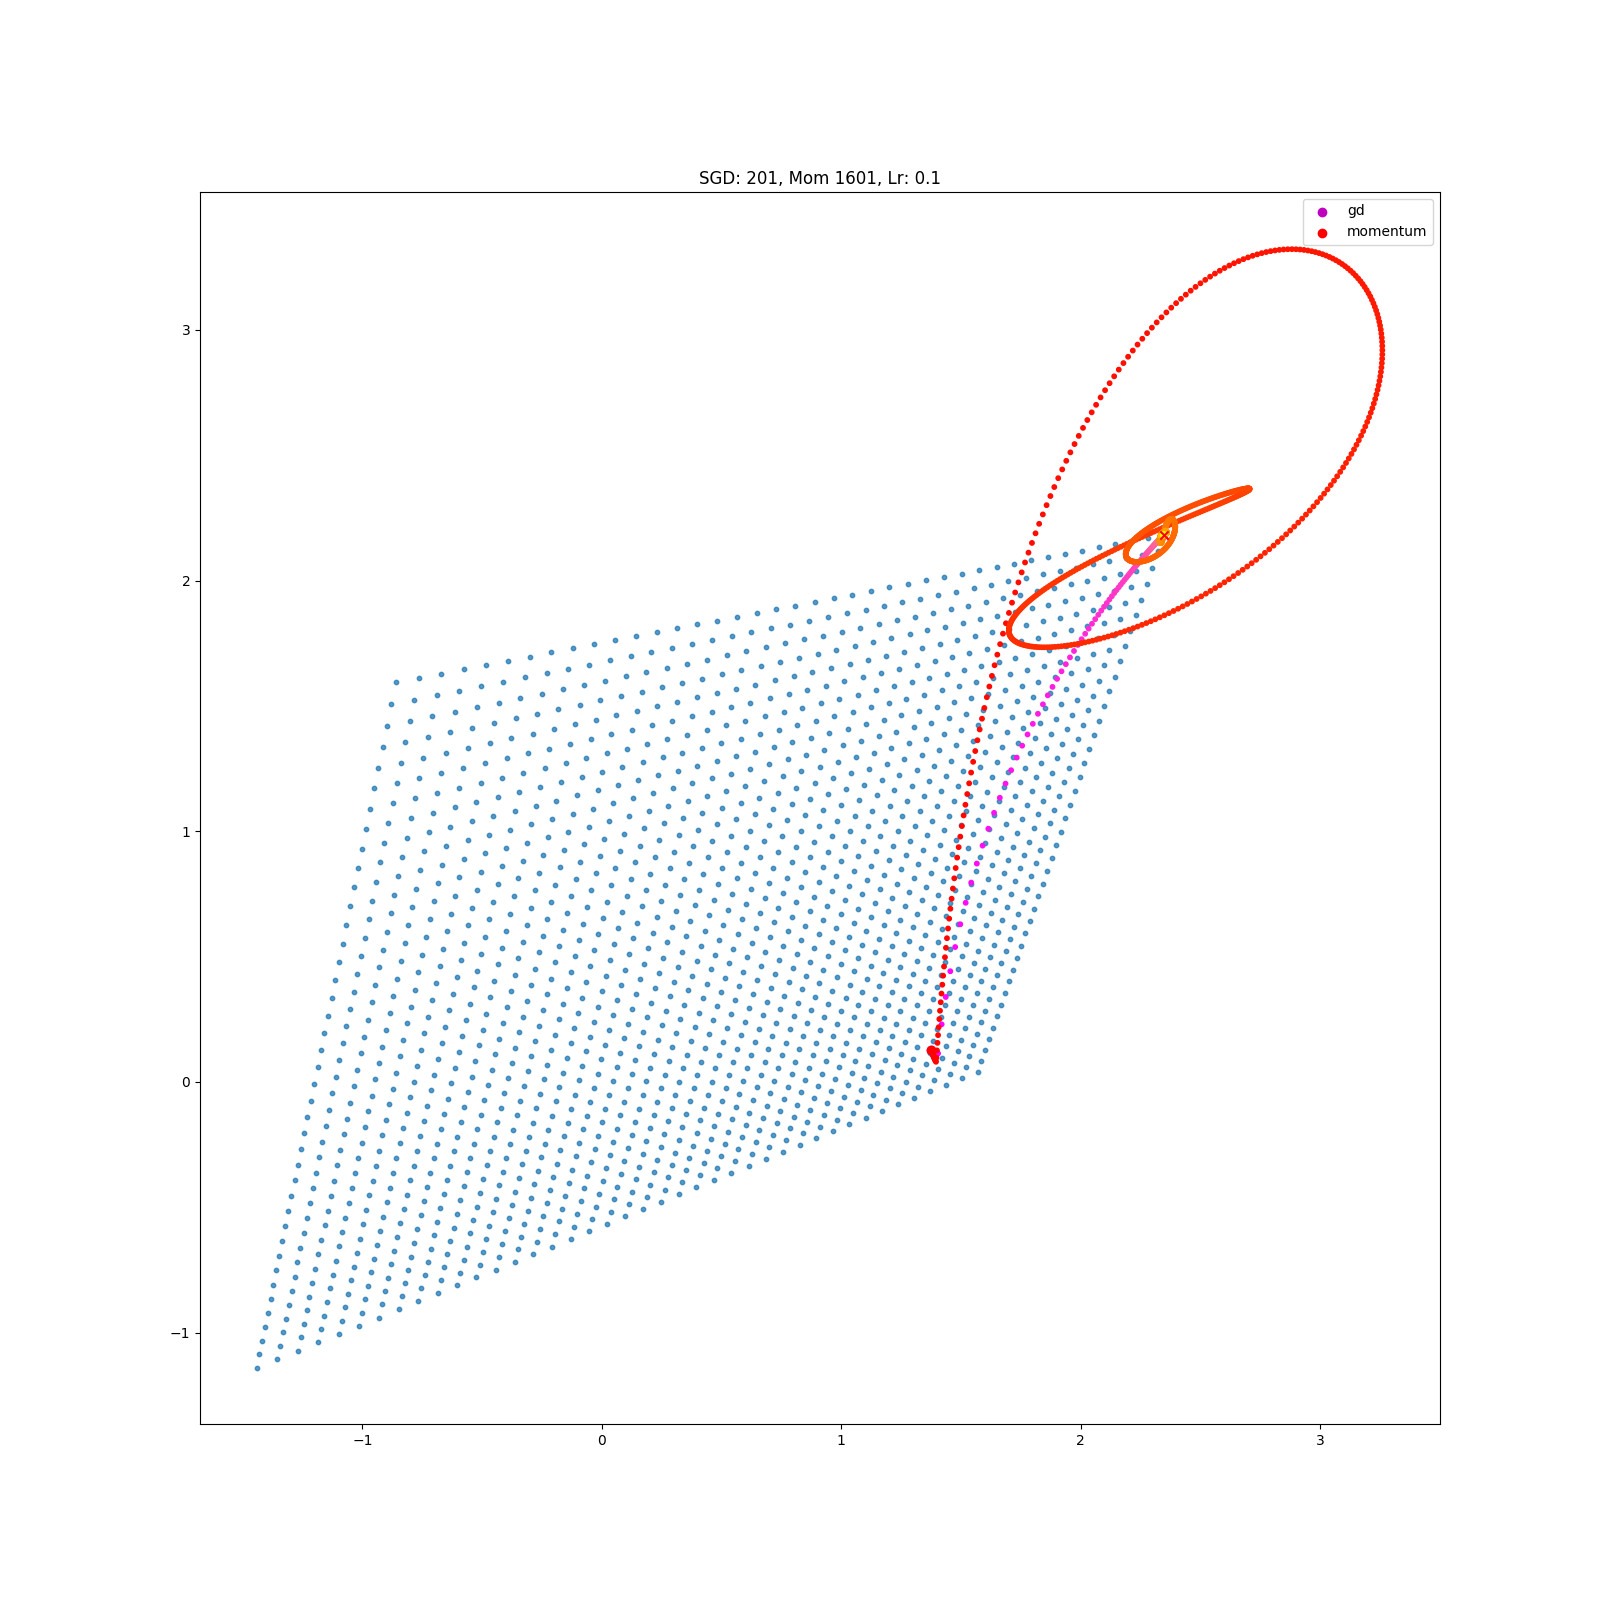
\includegraphics[width=0.5\textwidth,height=0.5\textheight]{../../pictures/figures/vi_sgd-vs-vi_mom_01.png}
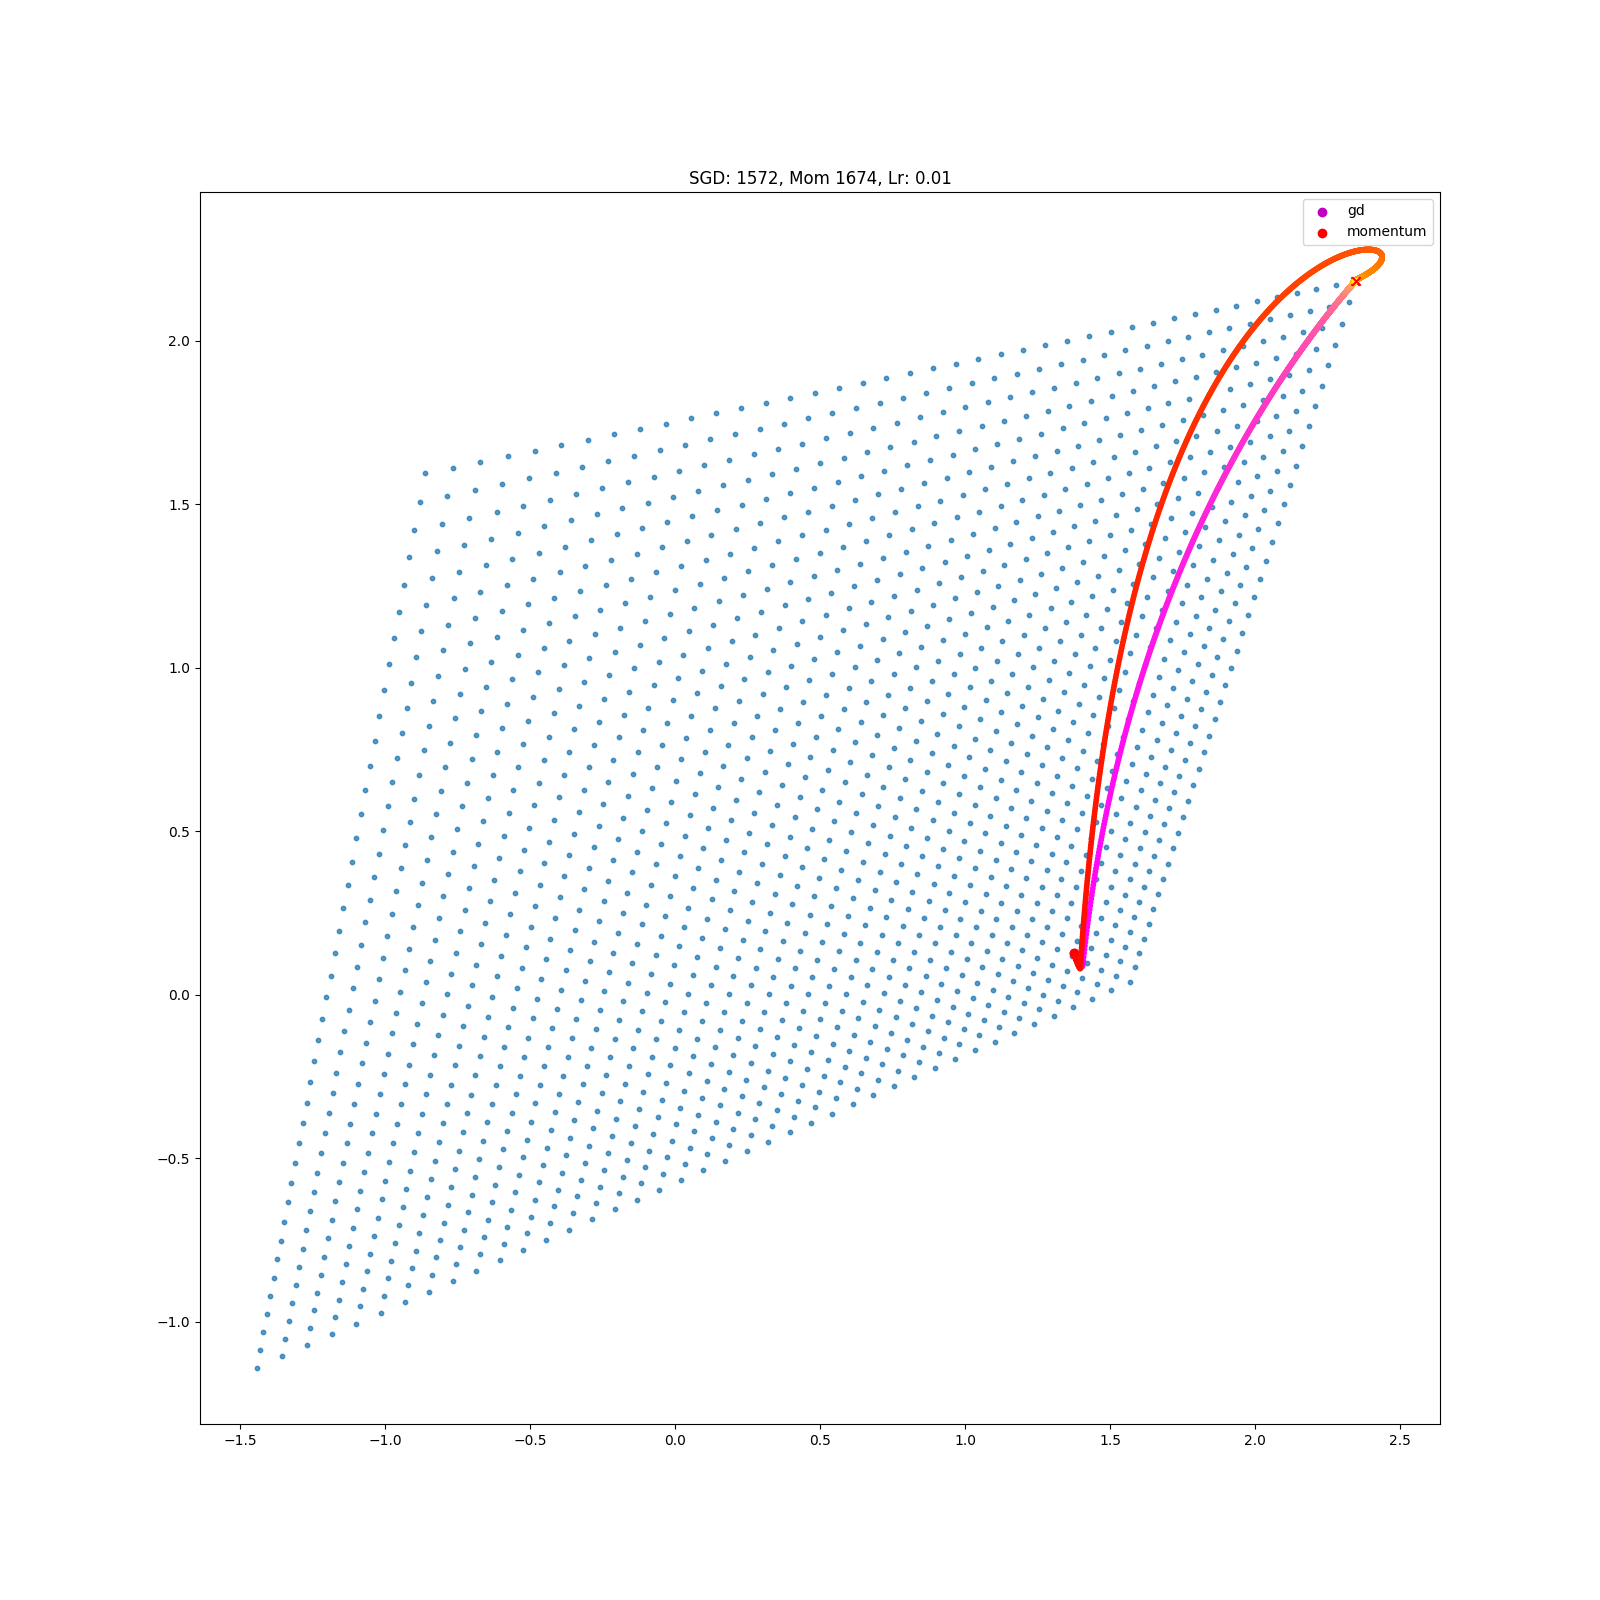
\includegraphics[width=0.5\textwidth,height=0.5\textheight]{../../pictures/figures/vi_sgd-vs-vi_mom_001.png}
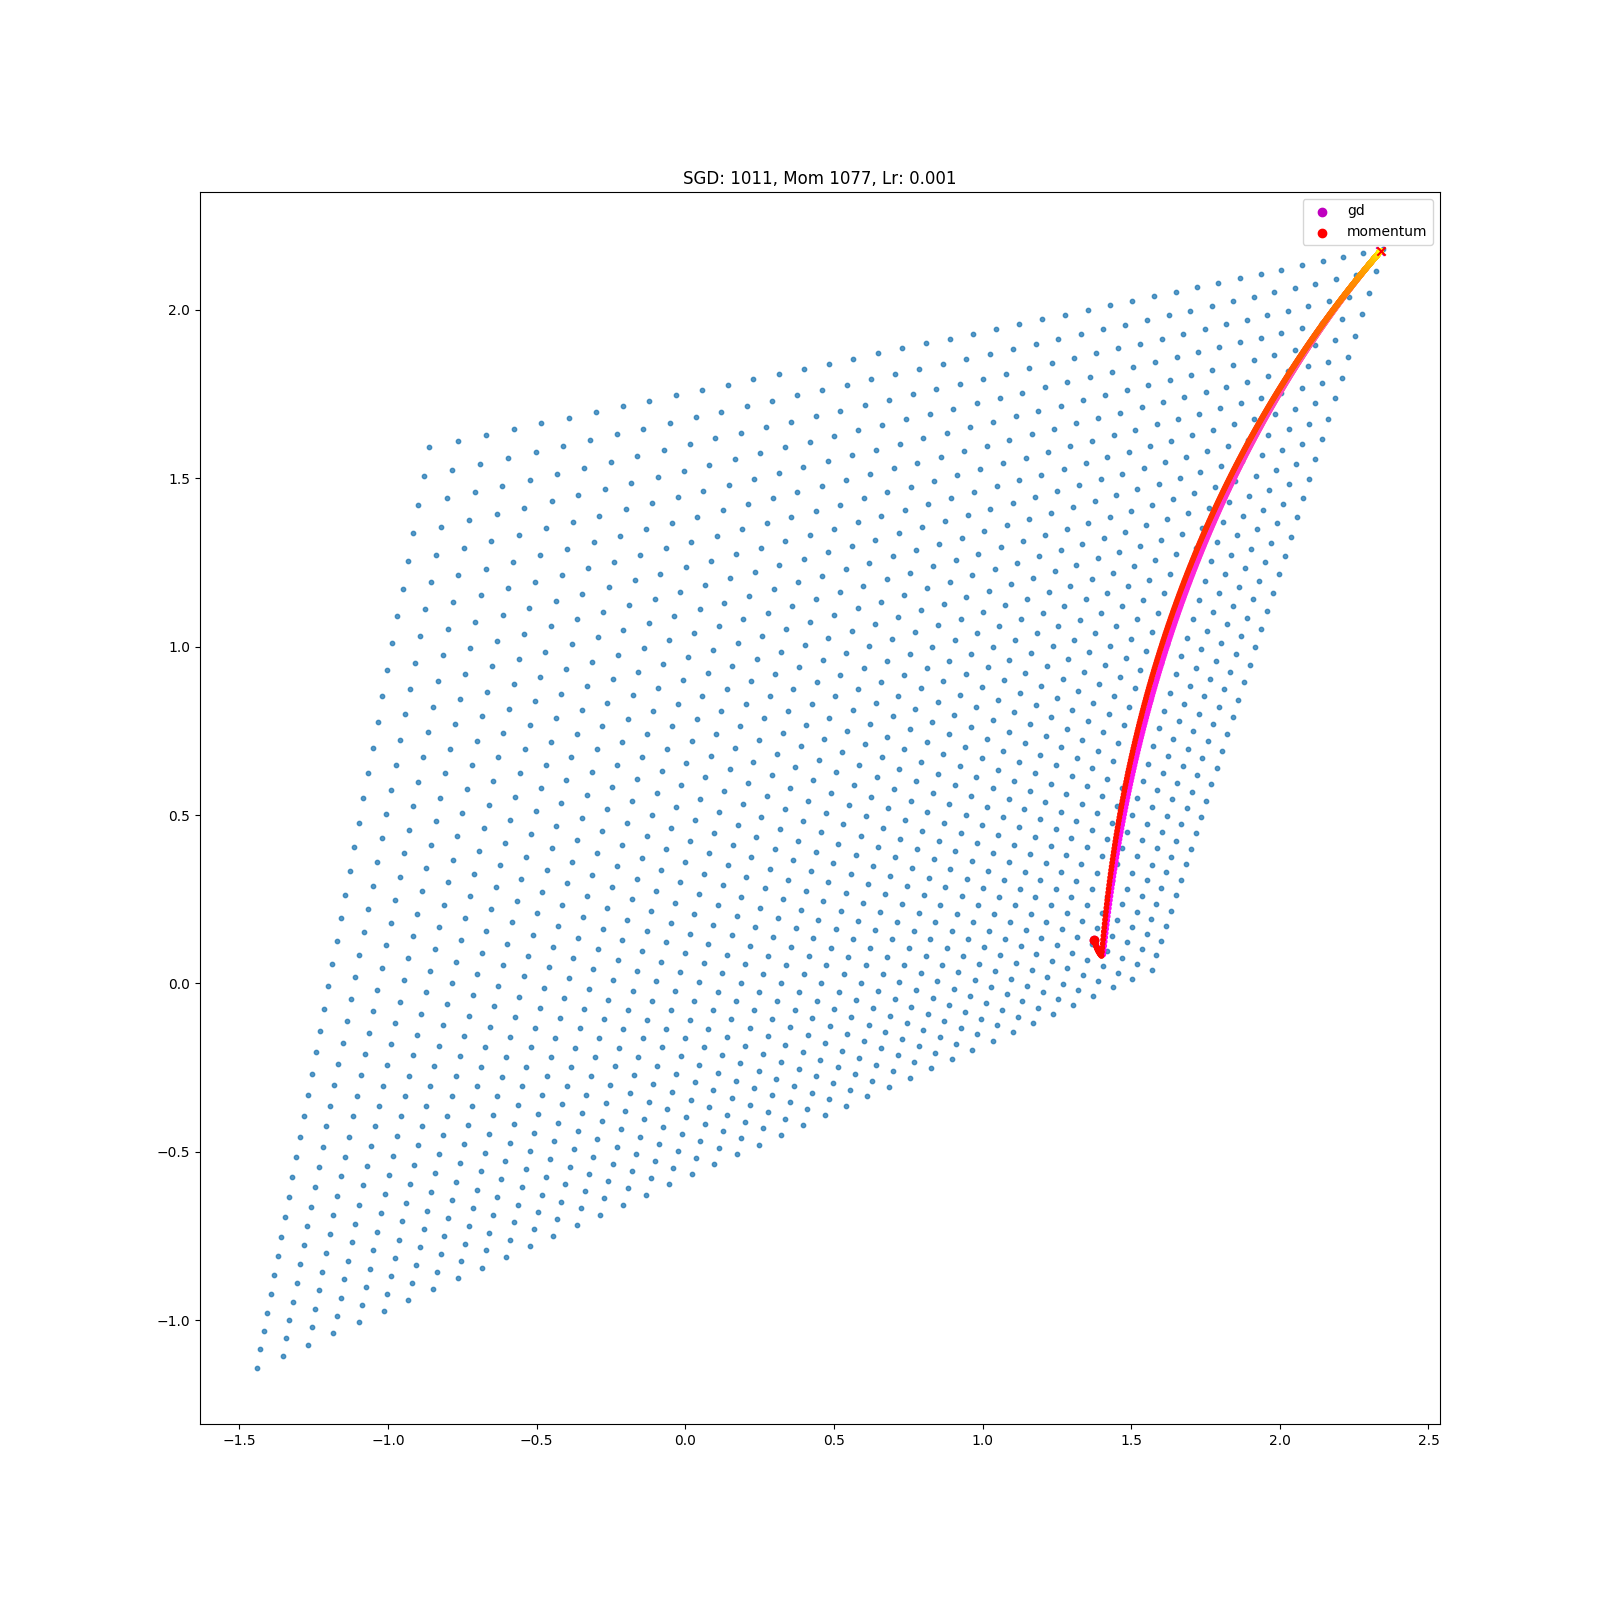
\includegraphics[width=0.5\textwidth,height=0.5\textheight]{../../pictures/figures/vi_sgd-vs-vi_mom_0001.png}

This is consistent with acceleration of gradient descent being a phenomena only possible in the discrete time setting. (see \cite{Betancourt2018} for a recent exploration)

This phenomena can be explained by the exponential decay of the momentum terms.

\begin{align}
m_{t+1} = m_t + \gamma\nabla f(w_t) \\
w_{t+1} = w_t - \eta (1-\gamma) m_{t+1} \\
\end{align}

As \(\eta \to 0\), \((1-\gamma) \cdot m_{t+1} \to \nabla f(w_t)\).

TODO, prove it.
